% 
% Annual Cognitive Science Conference
% Sample LaTeX Paper -- Proceedings Format
% 

% Original : Ashwin Ram (ashwin@cc.gatech.edu)       04/01/1994
% Modified : Johanna Moore (jmoore@cs.pitt.edu)      03/17/1995
% Modified : David Noelle (noelle@ucsd.edu)          03/15/1996
% Modified : Pat Langley (langley@cs.stanford.edu)   01/26/1997
% Latex2e corrections by Ramin Charles Nakisa        01/28/1997 
% Modified : Tina Eliassi-Rad (eliassi@cs.wisc.edu)  01/31/1998
% Modified : Trisha Yannuzzi (trisha@ircs.upenn.edu) 12/28/1999 (in process)
% Modified : Mary Ellen Foster (M.E.Foster@ed.ac.uk) 12/11/2000
% Modified : Ken Forbus                              01/23/2004
% Modified : Eli M. Silk (esilk@pitt.edu)            05/24/2005
% Modified : Niels Taatgen (taatgen@cmu.edu)         10/24/2006
% Modified : David Noelle (dnoelle@ucmerced.edu)     11/19/2014
% Modified : Roger Levy (rplevy@mit.edu)     12/31/2018



%% Change "letterpaper" in the following line to "a4paper" if you must.

\documentclass[10pt,letterpaper]{article}

\usepackage{cogsci}
\usepackage{url}

% \cogscifinalcopy % Uncomment this line for the final submission 


\usepackage{pslatex}
\usepackage{apacite}
\usepackage{float} % Roger Levy added this and changed figure/table
                   % placement to [H] for conformity to Word template,
                   % though floating tables and figures to top is
                   % still generally recommended!

%\usepackage[none]{hyphenat} % Sometimes it can be useful to turn off
%hyphenation for purposes such as spell checking of the resulting
%PDF.  Uncomment this block to turn off hyphenation.
\usepackage{graphicx}


%\setlength\titlebox{4.5cm}
% You can expand the titlebox if you need extra space
% to show all the authors. Please do not make the titlebox
% smaller than 4.5cm (the original size).
%%If you do, we reserve the right to require you to change it back in
%%the camera-ready version, which could interfere with the timely
%%appearance of your paper in the Proceedings.

\title{Birds and Words: Exploring environmental influences on folk categorization}
 
\author{{\large \bf Joshua T. Abbott (joshua.abbott@unimelb.edu.au)} \\
 {\large \bf Charles Kemp (ckemp@unimelb.edu.au)} \\
  School of Psychological Sciences,  \\
  University of Melbourne, 3010, Australia}



\begin{document}

\maketitle


\begin{abstract}

Anthropologists and psychologists have long studied how living kinds are organized into categories, and a recurring theme concerns the relationship between folk categories and the structure of the environment.  We ask whether the frequency and physical size of a species affects how it is classified, and address this question by linking frequency data from eBird (an online database of bird observations) with an existing taxonomy of Zapotec bird names.  A first set of analyses explores whether frequency and size predict whether a bird is named and how many other birds it is grouped with. A second set explores whether frequency and size predict the word forms used as category labels.  We find some evidence that frequency affects both category extensions and naming, but the results hint that frequency may be dominated by other factors such as perceptual similarity.  

%Questions of how categories of natural kinds are named have a long history in anthropology and psychology. There has been a particular debate over the influence of the external environment on how people partition the world. Recent large-scale digital datasets allow us to test old questions in a new light. In this paper we use frequency of occurrence and physical size of birds to examine the naming patterns of a folk categorization system. First, we explore the extensions of categories, and investigate whether these environmental factors predict whether a bird is named and how they are grouped with other birds by the same label. We then explore how the forms of category labels are predicted by the environmental factors. We find some evidence that frequency affects both category extensions and naming, but the results hint that frequency may be dominated by other factors such as perceptual similarity.
%We demonstrate that the recent development and release of multiple digital datasets allows us to investigate old questions with a new perspective.

\textbf{Keywords:} 
folk biology; ethno-ornithology; categorization; cognitive anthropology; bird naming
\end{abstract}


\section{Introduction}

Languages around the world include rich systems of names for plants and animals, and each system can be viewed as the outcome of a natural experiment in which generations of speakers have organized their local environment into categories. A classic line of work in cognitive anthropology addresses the question of how named categories reflect the structure of the local environment~\cite{berlin2014ethnobiological,malt95}. One prominent theme is that folk taxonomies often align well with Western scientific taxonomies, suggesting that folk taxonomies are shaped more by environmental structure than by the idiosyncratic needs and concerns of a particular culture \cite{berlin2014ethnobiological}

Much of the cognitively-oriented work on folk biology took place last century, and in recent years new data sets have made it possible to characterize the structure of the environment in ways that were previously difficult or impossible~\cite{sullivan2009ebird,wilman2014eltontraits}. Here we draw on these resources to revisit the classic question of the relationship between named categories and the environment. We focus on birds in particular, and begin by compiling properties of the bird species in a given area (e.g.\ how big is each species, and how often is it observed?) We then study how these properties relate to named bird categories in the local language. In particular, we ask whether the frequency of a species influences whether the species is named, and if so whether frequency influences the form of the name for that species and how many other species it is grouped with. 

The effects of frequency on categorization have been previously studied in the psychological literature~\cite{parducci83,nosofsky88,barsalouhl98}.  One relevant finding is that categories tend to be relatively broad in low-frequency regions of stimulus space, but relatively narrow in regions including frequently encountered stimuli~\cite{parducci83}. We might therefore predict that bird species encountered frequently are more likely to be assigned to their own distinctive categories.  

Our focus on frequency also connects with a prominent debate between \emph{intellectualist} ~\cite{berlin2014ethnobiological} and \emph{utilitarian} ~\cite{hunn1982utilitarian} accounts of folk classification. The intellectualist view holds that named categories reflect ``fundamental biological discontinuities'' that are perceptually salient (Berlin, 1992, p 53)~\nocite{berlin2014ethnobiological}, and assigns a minimal role to frequency. The utilitarian view emphasizes ways in which categories are useful for a given culture, and naturally accommodates frequency effects because assigning a label to a category is especially worthwhile if there are many occasions to use it.

The next section introduces the data sets that we use, and we then address two broad questions. First, we focus on category extensions, and ask whether environmental factors predict whether a species is named, and how the set of named species is organized into groups. Second, we focus on category labels, and ask whether environmental factors predict the relative lengths of category labels, and which labels have the structure of unmarked prototypes. 


\section{Data sets}

The literature contains detailed folk classifications of birds from several languages around the world, and we focus here on named bird categories from Zapotec \cite{hunn2008zapotec}, a language spoken in Oaxaca, Mexico.  We used two data sets that characterize the frequency and size of bird species found in Oaxaca, and a third that specifies how these species are organized into named categories.

\subsection{Frequency data}

Our frequency data are drawn from eBird, a citizen-science based bird observation network managed by the Cornell Lab of Ornithology \cite{sullivan2009ebird}.  eBird data are contributed by bird lovers (both professional and amateur) who use the site to record the time and place of bird sightings.  We used data from just the region containing the state of Oaxaca, Mexico\footnote{We used all eBird observation of frequency from the Basic Dataset (EBD) on https://ebird.org/data/download, last accessed January 24, 2020.}. An observer who sees a group of 5 vultures may record both the species (e.g.\ \emph{Cathartes aura}) and the number of birds in the group (5), but we treated each case like this as a single observation of the species in question. Our data for Oaxaca include 660,223 unique observations of 922 distinct species. 

We will take eBird counts as a very rough proxy for the frequency with which a species is encountered in the course of everyday life. The fact that nocturnal species will tend to have lower counts than equally common diurnal species is therefore a strength of the data rather than a limitation. eBird, however,  does not provide an unbiased measure of frequency in everyday life. As a group, eBird contributors are more interested in some species than others, and counts for rare but iconic species (e.g.\ the bald eagle in the USA) will overestimate the frequency with which they are encountered relative to other species. Even so, eBird is a valuable resource that allows rough estimates of a variable (frequency) that would otherwise be extremely difficult to measure.  


\subsection{Size data}
% Bird weights as an aid in taxonomy \cite{amadon1943bird}.
Beyond frequency it is plausible that physical and behavioral characteristics of birds both influence folk categorization. \citeA{hunn1999size} has documented that smaller species are more likely to be lumped together into large categories, and that larger species are more likely to be given distinct names. Following his lead we evaluate bird size as an influence on categorization, and use size data from EltonTraits~\cite{wilman2014eltontraits} which includes information on key attributes for all 9993 extant bird species, including those from Oaxaca.  We use the body mass variable, separately sourced from \cite{dunning2007crc}, which is defined as the geometric mean of average values provided for both sexes. Beyond body mass EltonTraits includes variables related to diet types, foraging strata, and activity patterns, and future studies can explore whether and how these variables influence naming. 

%\subsection{Phenotypic neighborhood}
%% Bird weights as an aid in taxonomy \cite{amadon1943bird}.
%
%An obvious factor affecting folk classification is that species are more likely to be grouped together if they look similar. We do not have detailed information about the appearance of species in our data set, but work with a similarity space (Figure~\ref{fig-morphospace}) that roughly captures similarity in physical appearance. \cite{pigot} generated a 9-dimensional morphospace based on body mass in addition to 8 variables related to beak shape and body shape, and we mapped their data down to the 
% 2 dimensional space in Figure~\ref{fig-morphospace} by running tSNE \cite{XXX}, an algorithm for dimensionality reduction. As with all tSNE solutions, the axes (and axis units) in Figure~\ref{fig-morphospace} cannot be precisely interpreted, but the x axis corresponds fairly closely to body mass (correlation is 0.96), and the isolated group of points at the far left ( \textit{dz\v{i}n\b{g}}) includes hummingbirds.  We used the space in Figure~\ref{fig-morphospace} to derive a neighborhood size score that counts the number of species within a distance of 0.5 units. The mean neighborhood size across all species in Figure~\ref{fig-morphospace} is 1.5, but the mean for the hummingbirds alone is 3.7.
%
%\begin{figure}[hbt!]
%  \begin{center}
%    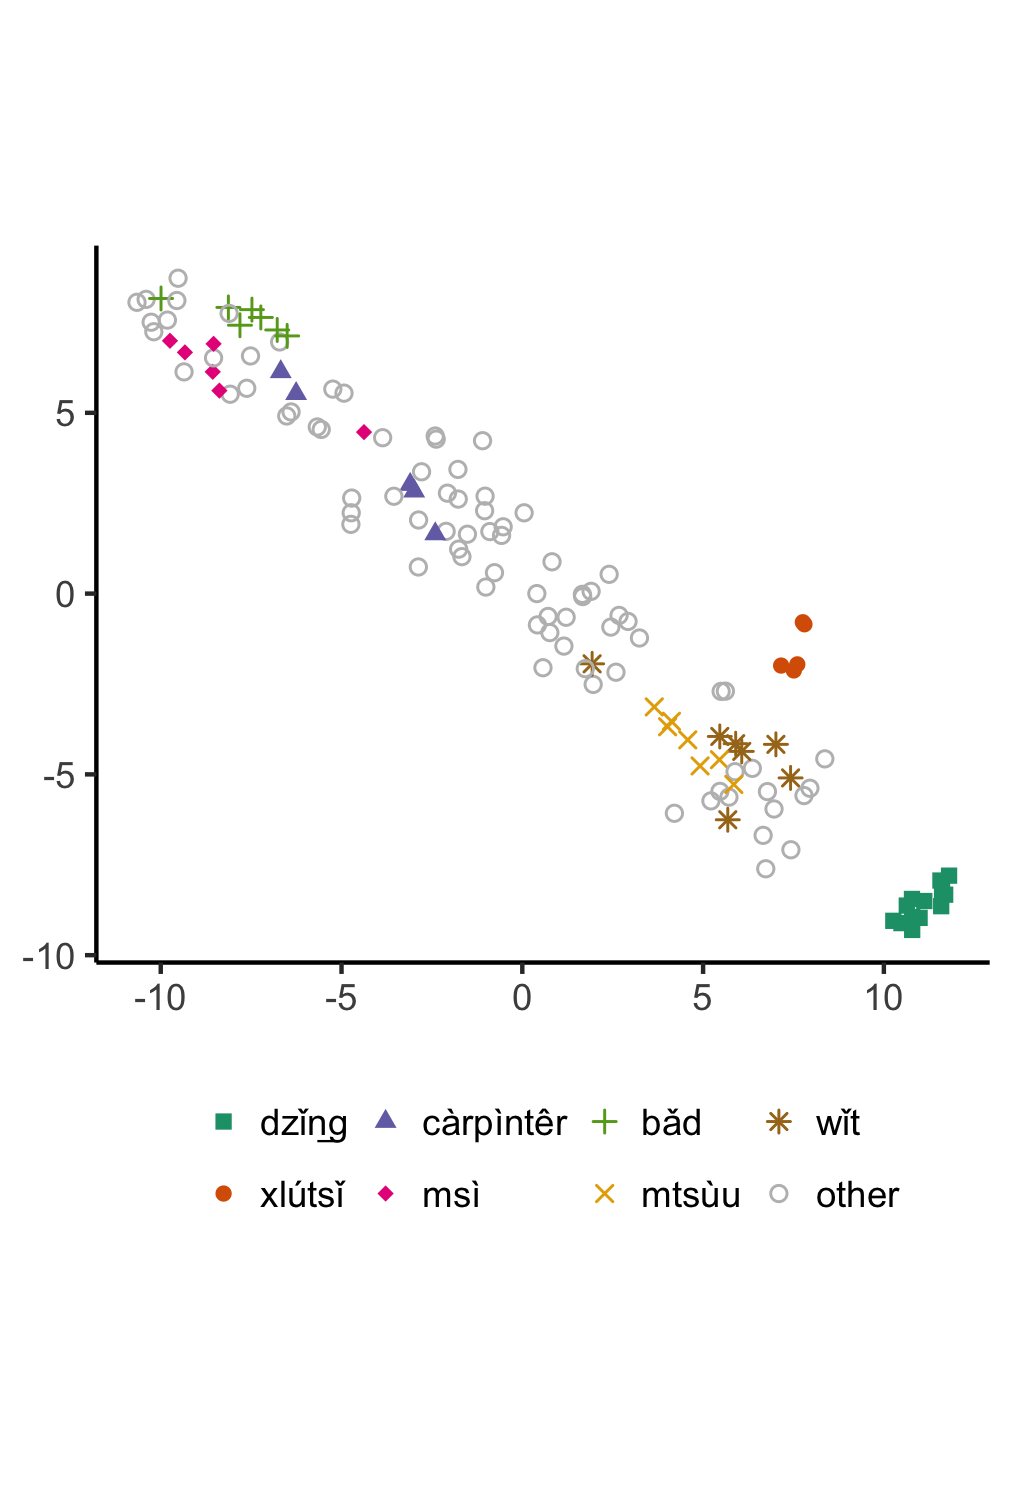
\includegraphics[width=3.375in]{./figures/morphospace.png}
%        \caption{Similarity space generated by applying tSNE to morphological data (e.g.\ beak shape, body shape and body mass). Colored points show species belonging to 7 Zapotec categories, and the remaining named species are shown as open grey circles.}
%        \label{fig-morphospace}
%  \end{center}
%\end{figure}


\subsection{Naming data}

Our naming data are based on a detailed folk taxonomy provided by \citeA{hunn2008zapotec} of the Zapotec language, from his fieldwork in San Juan Gb\"{e}\"{e}, a small village in Oaxaca, Mexico\footnote{ Also available online at \url{http://faculty.washington.edu/hunn/zapotec/z5.html}}. Folk classifications include names at different taxonomic ranks, and our data set includes a scientific name,  a folk-specific name and a folk-generic name for each species listed. For example, \emph{ Colibri thalassinus} (Mexican violetear) is named \textit{dz\v{\i}n\b{g}-y\v{a}-gu\`{i}} (mountain hummingbird) at the folk-specific level and \textit{dz\v{\i}n\b{g}} (hummingbird) at the folk-generic level.  According to Hunn's taxonomy the folk-generic category \textit{dz\v{\i}n\b{g}} (hummingbird) includes 14 different species. These 14 species are partitioned into 4 categories at the folk-specific level: \textit{dz\v{\i}n\b{g}}, \textit{dz\v{\i}n\b{g}-d\'{a}n-y\v{a}-gu\`{i}}, \textit{dz\v{\i}n\b{g}-gu\'{e}}, and \textit{dz\v{\i}n\b{g}-y\v{a}-gu\`{i}}.
As this example suggests, in some cases the folk-specific and folk-generic names for a species are identical: for example, 
 \emph{ Amazilia Beryllina} is known simply as \textit{dz\v{\i}n\b{g}} (hummingbird) at the folk-specific level.  %Following Hunn's usage any folk-specific category (e.g.\ the one that includes \emph{ Amazilia Beryllina}) with the same label as the folk-generic category to which it belongs will be called an \emph{unmarked prototype}.

In total Hunn's taxonomy includes 152 species that are organized into 94 distinct folk-specific categories, which in turn are organized into 69 folk-generic categories.  The scientific species labels given by Hunn did not always match those used by our other sources of data (eBird and EltonTraits).  We took the Clements checklist (used by eBird) as our gold standard \cite{clements2007clements}, and some manual preprocessing was required to align the labels used by all three resources.\footnote{All data and analysis code will be available on the first author's GitHub site.}



\section{Analysis of category extensions}

Given the three data sets just described we ask whether the frequency and body mass data can predict aspects of Hunn's naming data.  We focus first on the extensions of folk categories, and subsequently consider the labels or names given to these categories. 

Our first analysis considers whether frequency and mass can predict whether a species is likely to be named. Intuitively, one might expect that common species are more likely to be named, and that larger species are especially salient perceptually and therefore more likely to be named. Most descriptions of folk classification systems in the literature do not systematically describe species found in the local area that are \emph{not} named by the local people. Our eBird data, however, include species that were documented in Oaxaca but not included in Hunn's taxonomy. Some of these species are probably rarely if ever seen in the village (San Juan Gb\"{e}\"{e}) where Hunn carried out his fieldwork. We expect, however, that some species missing from the taxonomy would be occasionally encountered in San Juan Gb\"{e}\"{e}. 

\begin{figure*}[hbt!]
  \begin{center}
    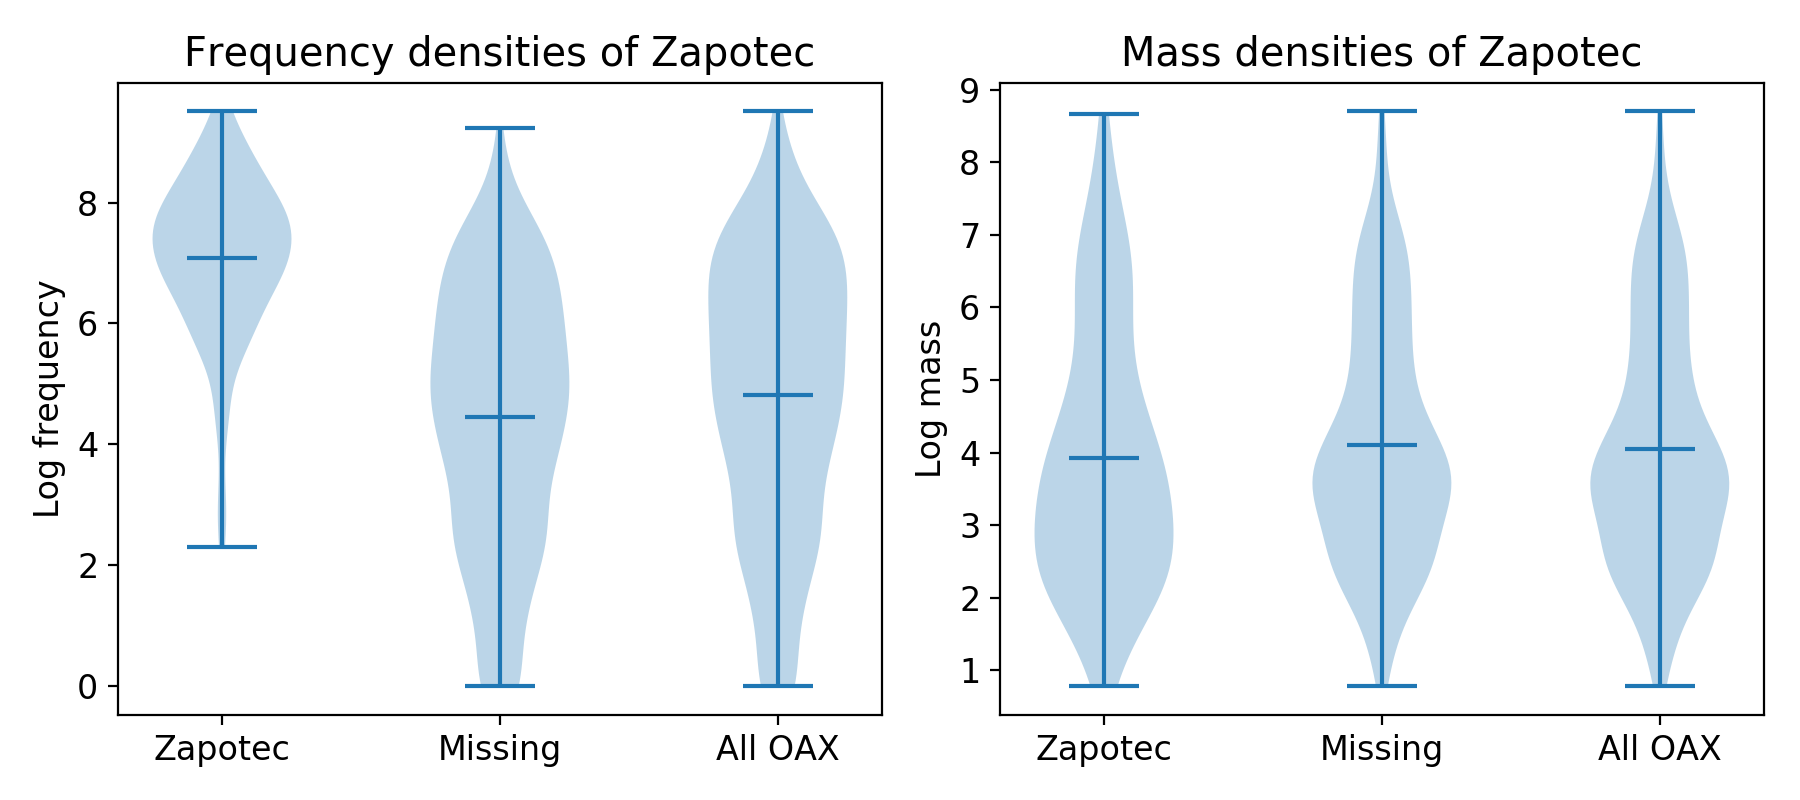
\includegraphics[width=.95\textwidth]{./figures/birdfreqmass-violinplots.png}
        \caption{Frequency densities (left) and Mass densitities (right) for species named in Zapotec, species found in Oaxaca (OAX) but missing from the Zapotec taxonomy, and all species in OAX.}
        \label{fig-birdfreqmassviolin}
  \end{center}
\end{figure*}

Figure~\ref{fig-birdfreqmassviolin} shows distributions of frequency and size for birds with and without Zapotec names.  As expected, on average birds that are named tend to be more frequent than birds that are not named. The mass distributions for named and unnamed birds, however, are very similar. To confirm these impressions we ran a logistic regression including log frequency and log mass as predictors of a binary variable that indicates whether a species was named. The estimated coefficients were $\beta = 0.84 \pm 0.09$ (log frequency) and $\beta = -0.03 \pm 0.07$ (log mass). Based on these coefficients, if the probability that a species would receive a name were initially 0.5, increasing the log frequency of the species by one unit would increase the naming probability to 0.65, and increasing the log mass by one unit would decrease the naming probability to 0.49. We compared the full logistic regression model to alternatives that removed either log frequency or log mass as a predictor, and found that removing log frequency produced a significant impairment ($\chi^{2}(1) = 137.04, p < 1e-10$), but removing log mass did not ($\chi^{2}(1) = 0.29, p = 0.59$).  Akaike information criterion (AIC) scores supported the conclusion that the model with log frequency but without log mass is the best among the three. 

% mention that information about unnamed species not systematically included in folk taxonomies



\subsection{Category size}


Next we explore how named species are organized into categories. In particular, we explore whether the frequency and mass of a species partially predict the number of other species it is grouped with at the folk-generic level.  Following prior work on frequency effects in the experimental literature~\cite{parducci83}, we hypothesized that frequent species would tend to be grouped with fewer others, because investing in a distinctive name for a species makes most sense if there are many occasions to use it. We also expected to replicate the work of \citeA{hunn1999size}, who reported that larger species tend to be grouped with fewer others, which makes sense given that larger species are especially salient perceptually. 

\begin{figure*}[!ht]
  \begin{center}
    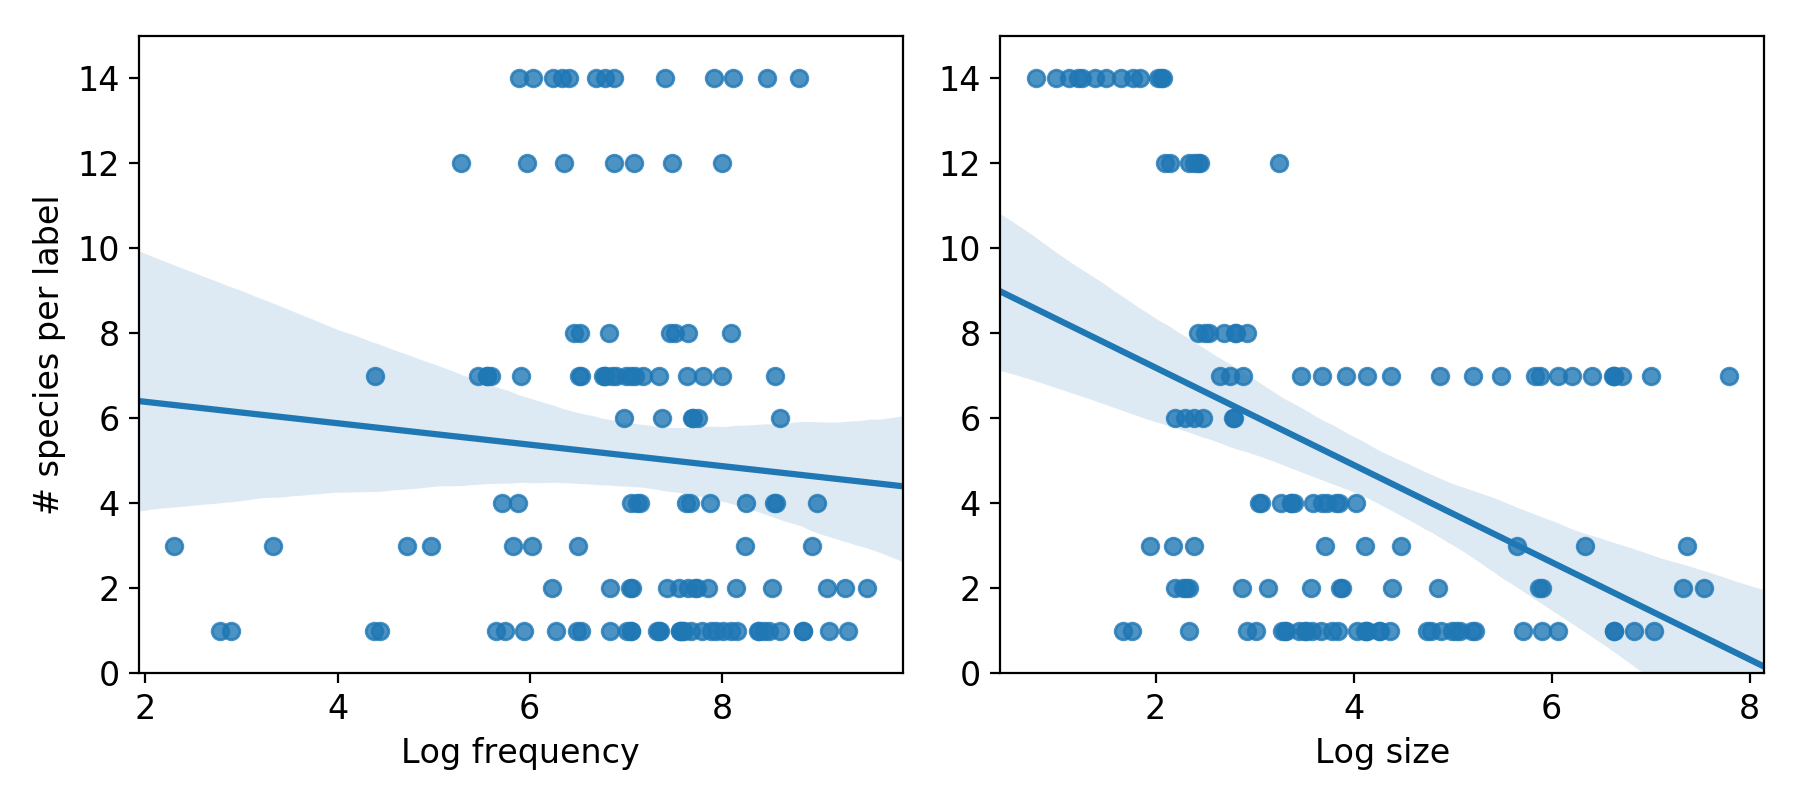
\includegraphics[width=0.90\textwidth]{./figures/ssrr-singlespecies.png}
    \vspace{-0.1in}
        \caption{Category size plots for both frequency (left column) and mass (right column). Category size is defined as the number of other species a bird is grouped with under the same folk-generic name. Each point represents a bird species named in Zapotec.}
        \label{fig-ssrr}
  \end{center}
\end{figure*}

The \emph{category size} of each species is defined as the total size of the folk-generic category to which it belongs. For example, \emph{ Colibri thalassinus} (Mexican violetear) is grouped with 13 other species called \textit{dz\v{\i}n\b{g}} (hummingbird) at the folk-generic level, and therefore receives a category size of 14.  Figure~\ref{fig-ssrr} shows plots of category size (at the folk-generic level) against both frequency and mass, and shows that mass is a stronger predictor ($r^2 = 0.20$) than frequency ($r^2 = 0.01$). The coefficients of a linear regression also suggest that mass ($\beta = -1.23 \pm 0.21$) is a stronger predictor than frequency ($\beta = -0.55 \pm 0.26$). Comparing the full model with both predictors to models that remove one predictor, however, suggests that removing mass significantly impairs the fit of the model ($\chi^{2}(1) = 513.87, p < 1e-5$), as does removing frequency ($\chi^{2}(1) = 65.05, p < 0.05$). AIC values support this same conclusion.

Overall these findings support Hunn's finding that larger species tend to be assigned to smaller categories, but suggest that frequency predicts category size only weakly. Our analyses, however,  did not include a third environmental factor  which probably interacts with body mass and frequency. The category size of a species almost certainly depends on how many other similar species are found in the environment. For example, one reason why \textit{dz\v{\i}n\b{g}} (hummingbird) is the largest folk-generic category in our data is that Oaxaca has many species of hummingbirds that look relatively similar to each other and relatively distinct from other species in the environment. In preliminary work we attempted to formalize this idea using a similarity space based on data from \citeA{pigot2020macroevolutionary}, who generated a 9-dimensional space that includes most of the world's bird species and is based on body mass in addition to 8 variables related to beak shape and body shape. We extracted a subset of this space that included only species named in Zapotec, and defined a \emph{neighborhood density} measure that captures the number of species that lie within a small radius of each point in the space. We found that neighborhood density predicted category size about as strongly than mass, but that body mass and frequency remained significant as predictors even when neighborhood density was included. In future work we plan to follow up on this preliminary result by evaluating models of unsupervised categorization that are defined over the similarity space. Some of these models are sensitive to both similarity and frequency, and therefore provide a natural way to explore how the two may interact in shaping folk categorization systems.

\section{Analysis of category labels}

The previous section focused on category extensions, but we now ask whether frequency and mass influence the form of the names for each species. We focus on names at the folk-specific level and consider three lexical properties of these names: name length, whether the name is a compound or monomial, and whether the name is an unmarked prototype.

\subsection{Name length}

Zipf's law (1936, 1949)\nocite{zipf1936psycho,zipf1949human} is the well-established regularity that word lengths are  inversely related to word frequency. Intuition suggests that the frequency with which a species is named should roughly track the frequency with which it is observed, and we therefore hypothesized that more frequent species would tend to have shorter names.  In contrast, we expected that there would be no relationship between body mass and name length. 

Because we do not have phonemic representations of the Zapotec names, we used a crude measure of length based on the number of characters in the written form of each name. We analyzed both the frequencies and masses of birds named in Zapotec in relation to the name length of the bird. In a direction opposite to our predictions, birds with longer names had a slight tendency to be more frequent, while having a slight tendency to be of smaller size. However, the coefficients of a linear regression suggest that log frequency ($\beta = 0.04 \pm 0.03$) and log mass ($\beta = -0.06 \pm 0.03$) are both weak predictors of log name length. Comparing the full linear regression model with both predictors to alternatives that dropped mass as a predictor significantly impaired model performance ($\chi^{2}(1) = 1.28, p < 0.02$) but dropping frequency did not ($\chi^{2}(1) = -0.39, p < 0.2$). AIC scores support the same conclusion.


\subsection{Compound names}

As suggested earlier, some hummingbirds have compound names at the folk-specific level (e.g.\ \textit{dz\v{\i}n\b{g}-y\v{a}-gu\`{i}} (mountain hummingbird)) but others do not (e.g.\   
\emph{ Amazilia Beryllina} is known simply as \textit{dz\v{\i}n\b{g}} (hummingbird)). Compound names are notated in Hunn's taxonomy with a dash ('-'), and we explored whether frequency and mass could predict whether the folk-specific name for a species is compound or monomial. 


%When analyzing the densities of monomials to compounds, we found both distributions in both cases are similar. 
Compounds tend to be longer than monomials, and consistent with our analysis of name lengths we found 
that neither log frequency nor log mass predicts whether a species has a monomial name. The coefficients of a logistic regression suggest that log frequency ($\beta = -0.10 \pm 0.14$) is a stronger predictor than log mass ($\beta = -0.03 \pm 0.11$), and that as the frequency or mass of a species increases it becomes less likely to have a compound name. However, comparisons of the full model to alternatives that remove either log frequency or log mass  suggest that neither predictor is significant ($\chi^{2}(1) = 0.55, p = 0.46$ for log frequency and $\chi^{2}(1) = 0.08, p = 0.78$ log mass).  AIC scores support the same conclusion. 


\subsection{Prototypes}
% 5b) pěch-rúx [`vulture´ + `naked´] (= ngól̲-běts [X + Y]); Black Vulture (Coragyps atratus): less common and widespread than the next; the generic synonym was reported by Reeck;
% 5c) pěch[-0] [`vulture´, unmarked prototype] (= pěch-yèts [`vulture´ + `yellowish´]); Turkey Vulture (Cathartes aura): the prototypical vulture; normally simply named pěch.
% XXX: replace hummingbirds with another example that's actually in the plot

\begin{figure*}[ht!]
  \begin{center}
    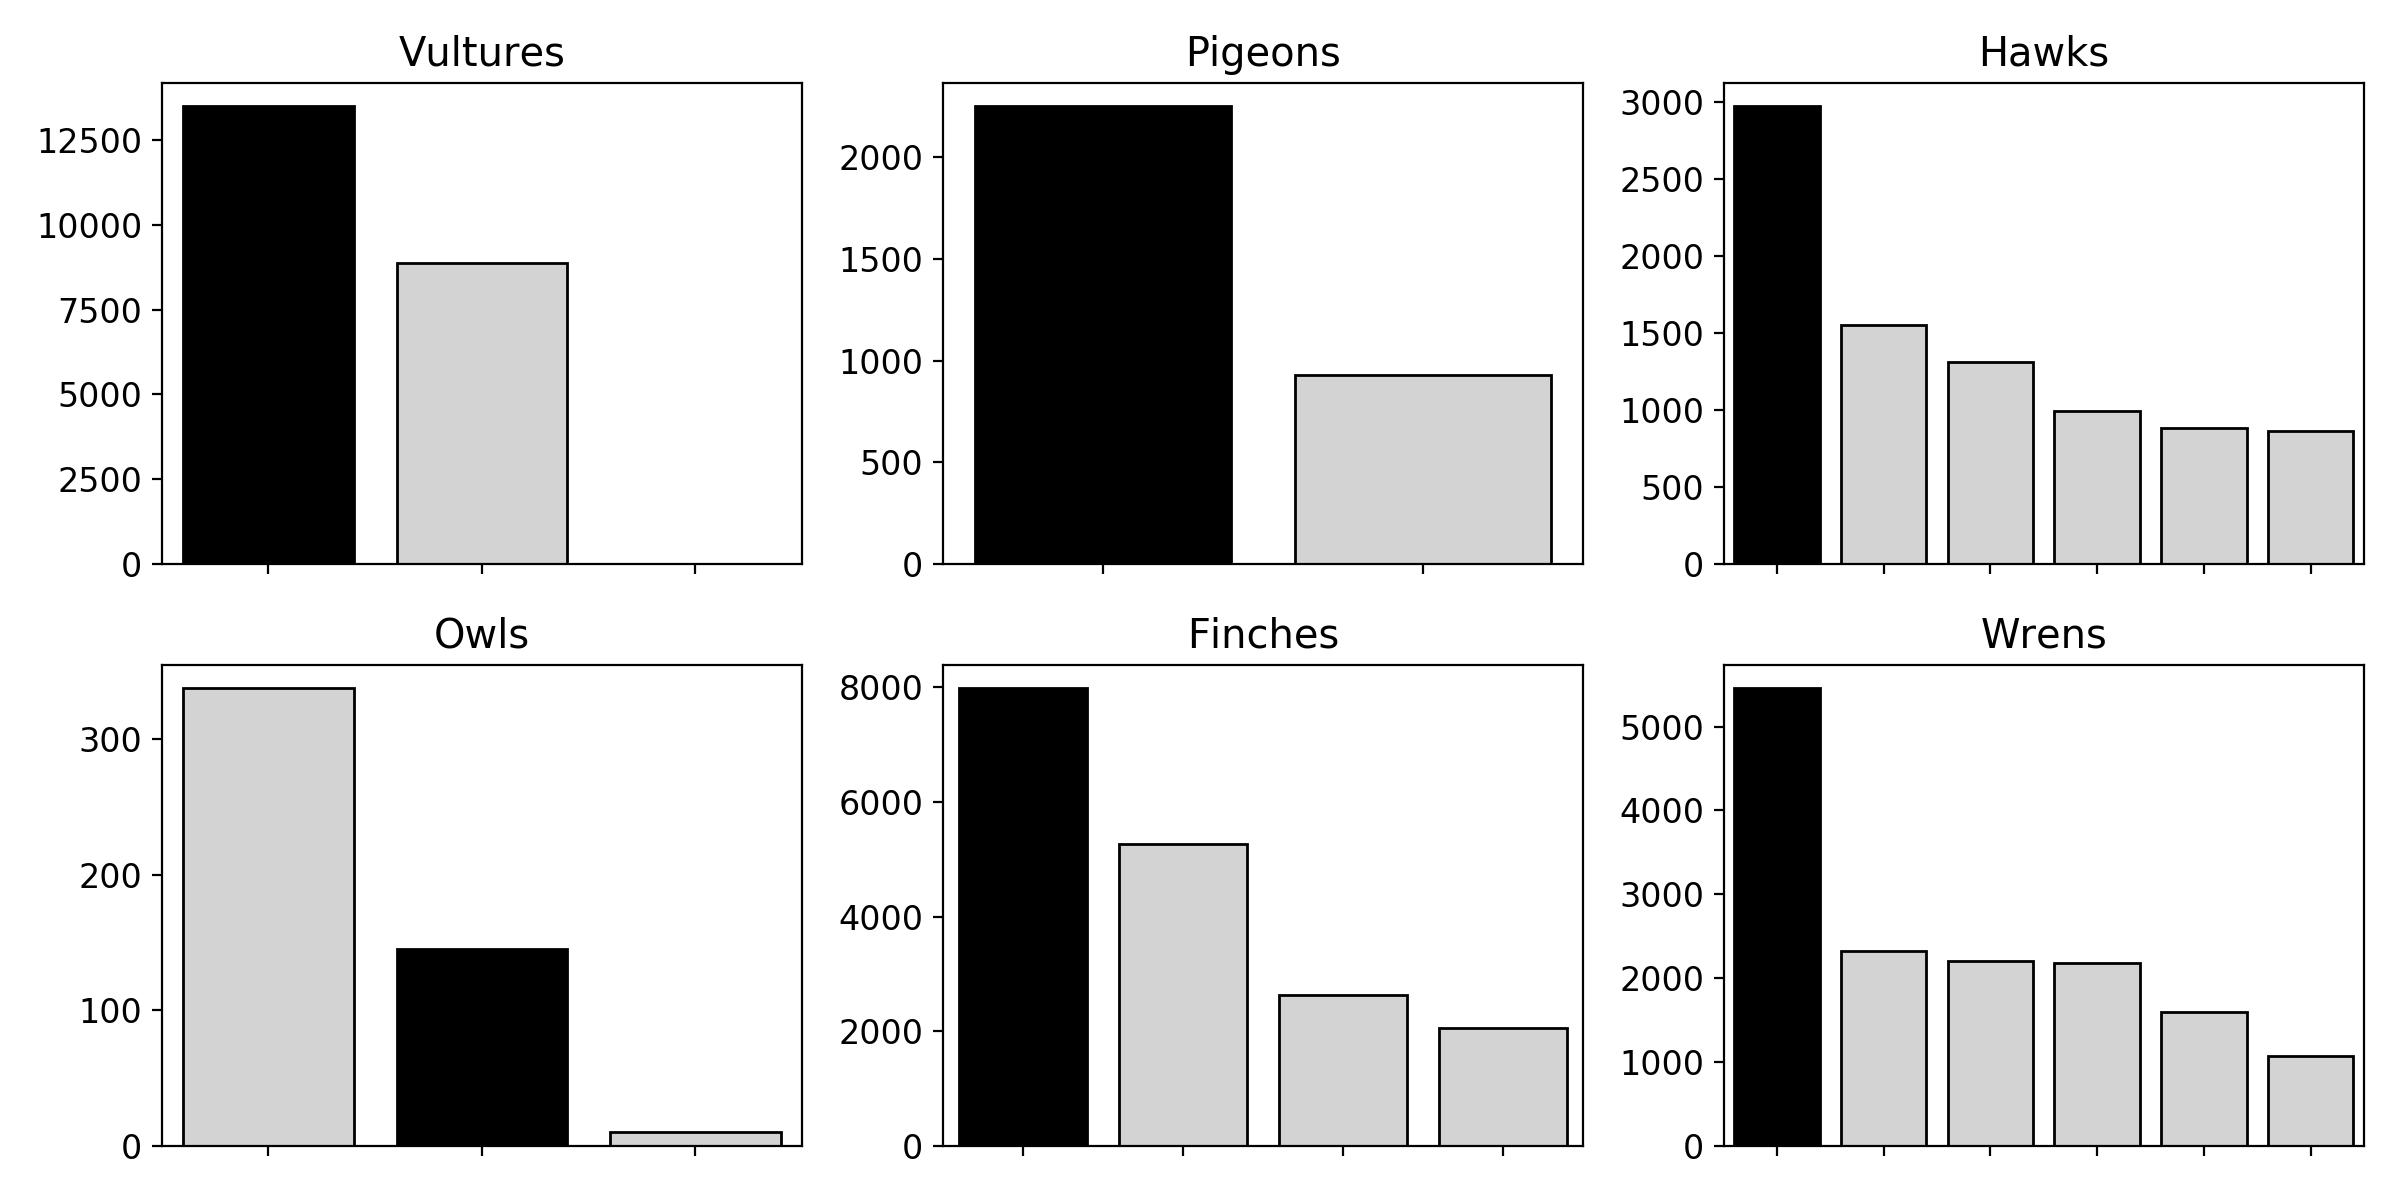
\includegraphics[width=0.95\textwidth]{./figures/prototypes-barplots-all.png}
    \vspace{-0.05in}
        \caption{Frequency bar plots of birds named in Zapotec as unmarked prototypes along with frequencies of other birds with the same folk-generic name. The bar highlighted in black is the unmarked prototype.}
        \label{fig-freq-prototype-all}
  \end{center}
\end{figure*}

The literature on folk categorization proposes a link between monomial labels and category prototypes
~\cite{berlin1972speculations,berlin2014ethnobiological}. If some vultures (e.g.\ Turkey vulture, \emph{ Cathartes aura}) are simply called \textit{p\v{e}ch} at the folk-specific level but others have a compound name (e.g.\ \textit{p\v{e}ch-r\'{u}x}, or Black vulture), then vultures with the monomial name might be expected to be more typical than those given a distinctive folk-specific name. Several factors could contribute to typicality: for example, typical vultures could be those encountered most frequently, or those that are perceptually most representative of the folk-generic category 
\textit{p\v{e}ch} \cite{berlin2014ethnobiological}.  Here we test the hypothesis that frequency predicts typicality.

For us, any folk-specific category (e.g.\ the one that includes \emph{ Cathartes aura}) with the same label as the folk-generic category to which it belongs will be called an \emph{unmarked prototype}.  Although this definition of a prototype is based purely on linguistic form, we expect that it lines up with the psychological notion of a prototype~\cite{rosch73}. Hunn's data includes 11 unmarked prototypes, and for simpilicity we focus on the 6 prototypes that include a single species each, which means that the species in question can be treated as a category prototype.

Figure \ref{fig-freq-prototype-all} shows ranked raw frequency distributions that compare the frequency of each category prototype to the frequency of other members of the same folk-generic category. 
The top left chart indicates that the prototypical Turkey Vulture (in black) is more frequently observed in Oaxaca than other vultures. This trend holds across 5 of the 6 cases, with a notable exception for the folk-generic category including owls. Although the counts for this category are comparatively low, the unmarked prototype (Great Horned Owl) is only the second most frequent owl in the eBird data. Hunn notes that the Great Horned Owl is considered an ill-omen by many, and the cultural salience of this species may therefore explain why it receives an unmarked name despite being infrequently observed. 


% \begin{figure*}[ht!]
%   \begin{center}
%     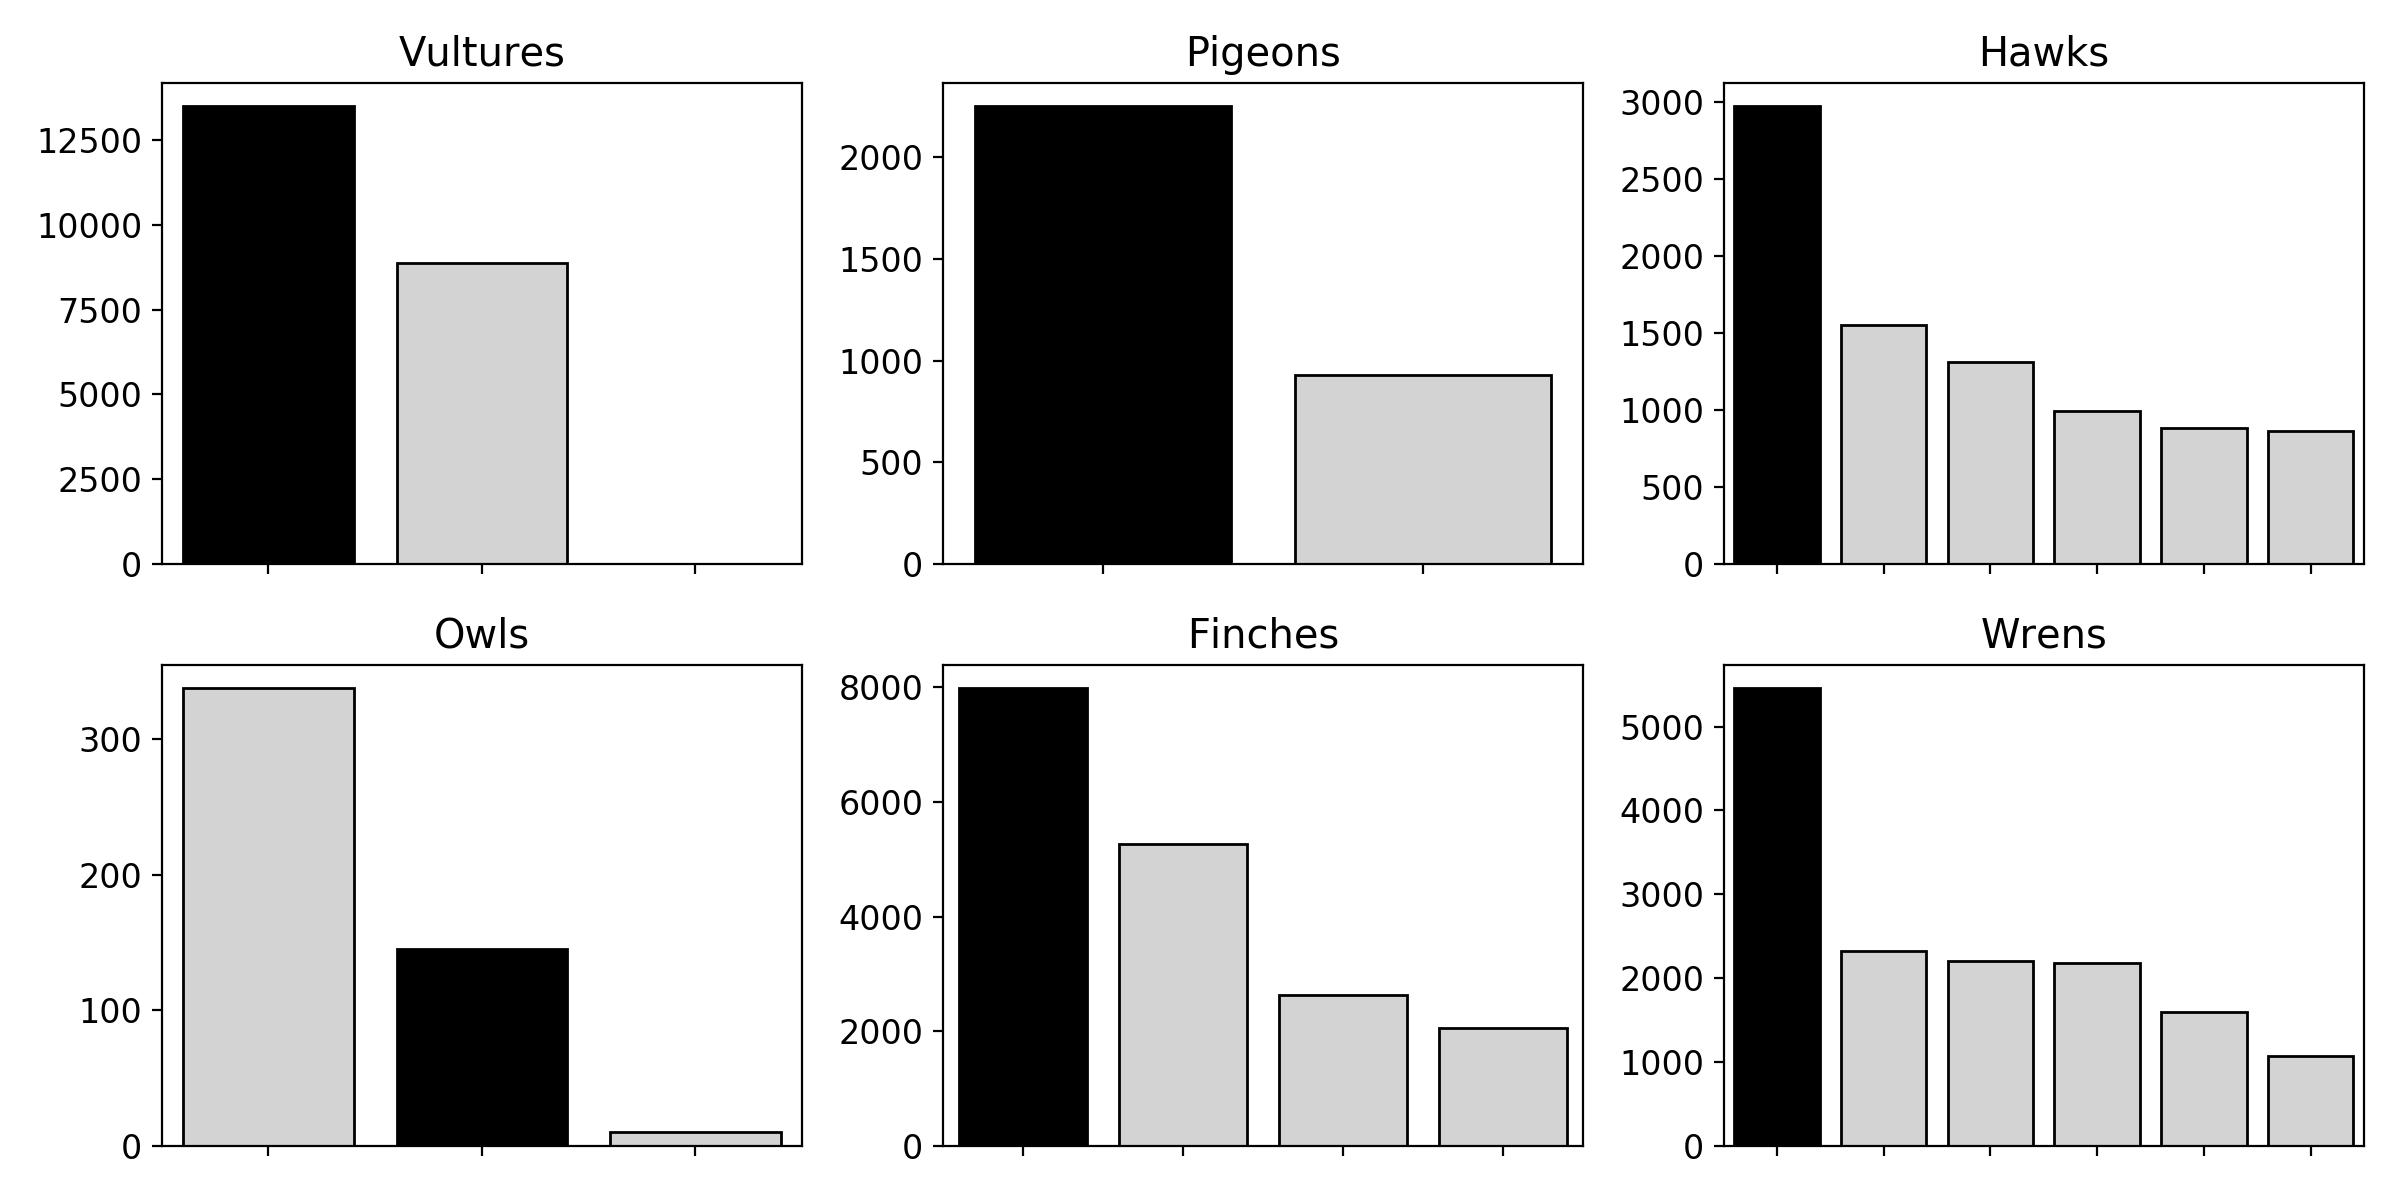
\includegraphics[width=0.95\textwidth]{./figures/prototypes-barplots-all.png}
%         \caption{Frequency bar plots of birds named in Zapotec as unmarked prototypes and the frequencies of other birds with the same folk-generic name. The bar highlighted in black is the unmarked prototype.}
%         \label{fig-freq-prototype-all}
%   \end{center}
% \end{figure*}


\section{Discussion}

% Summary of some of the questions we could explore using the methods detailed above.

% themes:
% experimental vs naturalistic research (tight control on similarity)

We drew on large-scale digital data sets to ask whether the physical size of a bird species and its frequency of occurrence predict how it is classified in a Zapotec folk taxonomy.  Our first set of analyses found that frequency (but not mass) predicts whether or not a species is named, and that both frequency and mass predict category size (i.e.\ how many other species a given species is grouped with at the folk-generic level). Hunn previously reported that mass predicts category size, and we found mass to be a stronger predictor than frequency. The relatively weak effect of frequency may seem at odds with previous experimental studies that report strong effects of frequency on categorization~\cite{parducci83}. Experimental work, however, is often able to tightly control stimulus similarity, but we analyzed biological species that belong to a similarity space with rich naturalistic structure. Although perceptual similarity and frequency both affect categorization, the weak effect of frequency in our category size analysis suggests that perceptual similarity may be the stronger of the two factors.  

%First, observation frequency (how often a species is seen) is not the same as communication frequency (how often a species is talked about). 

Our second set of analyses focused on category names. Although our results suggest that frequency influences some aspects of naming (e.g.\ whether the folk-specific name for a species is an unmarked prototype), to our surprise, we found that frequency did not predict the length of a species' name, or whether the name is compound or monomial. Two possible explanations seem plausible. Consistent with Zipf's law, it is possible that frequently used names do tend to be short, but that these names do not pick out the species that are observed most frequently. Commonly discussed species may include cases (e.g. the bald eagle in American culture) that have cultural significance even though they are observed relatively rarely. The second possible explanation is that the effect of frequency is again dominated by perceptual similarity. For example, compound names may be most useful in ``crowded'' regions of perceptual space where they can serve to distinguish one species from its neighbors. In extreme cases where a species (e.g.\ the Australian emu) is the only member of a folk-generic category, there is no reason to give it a compound name at the folk-specific level regardless of how frequently the species is observed. 

Frequency plays a central role in theories of communicative efficiency. For example, efficiency-based theories of categorization predict narrow categories in frequently-observed regions of stimulus space~\cite{regierck16}, and Zipf's law can be explained in terms of communicative efficiency~\cite{ferrericanchos03}. In turn, the notion of communicative efficiency is linked with the utilitarian approach to folk classification~\cite{hunn1982utilitarian}, which suggests that folk categories are best understood by explaining the purpose they serve in a given culture. Our results, however, suggest that frequency-related effects may be dominated by perceptual similarity. If supported in future work this conclusion would be broadly compatible with the intellectualist account of folk classification~\cite{berlin2014ethnobiological}, which focuses on perceptual salience rather that communicative utility. A pressing goal for future work is to combine our frequency data with a perceptual similarity space derived from \cite{pigot2020macroevolutionary} and to explore whether and how the two interact in shaping folk classification. 

A second important goal for future work is to expand our approach to languages other than Zapotec. The best candidates are languages for which a reliable folk taxonomy is available and for which eBird data  
is relatively plentiful for the geographic region in question.  Clear next steps are to analyze folk taxonomies for Tzeltal (Chiapas, Mexico)  and Tlingit (south-east Alaska)~\cite{hunn1977tzeltal,hunn2012tlingit}.

%both published by Hunn as well \cite{hunn1977tzeltal,hunn2012tlingit}, which have decent coverage within their respective geographics regions in eBird observational data. 

%That said, it can be difficult to find languages with both expert ethnographries of the folk biological naming systems which also have good coverage in eBird. This has prohibited us from exploring bird naming data from known experts in regions with low coverage in eBird (e.g., naming data summarized in \cite{holman2002relation}, including the Tobelo language from Indonesia \cite{taylor1990folk} and the Anindilyakwa language from Australia \cite{waddy1988classification}, which do not have coverage in eBird currently).



%Questions of how categories of natural kinds are named have a long history in anthropology and psychology. There has been a particular debate over the influence of the external environment on how people partition the world. Recent large-scale digital datasets allow us to test old questions in a new light. In this paper we use frequency of occurrence and physical size of birds to examine the naming patterns of a particular folk categorization system. We found evidence that frequency predicts whether or not a species is named, and when a species is an unmarked prototype, as well as weak evidence that it predicts lumping. We replicated \citeA{hunn1999size} and found size predicts lumping (and find that it's a stronger predictor than frequency), but found only weak evidence that it predicts anything else.

%Reasons why we don’t see a stronger effect of frequency (discuss wrt theories that do predict frequency effects including functional/utilitarian view, Zipfian view, perhaps others)

%Distribution of species in morphospace is an important confound in lumping, compound vs monomial and namelength analyses. Possible that similarity is the big thing: e.g if a species is very similar to many other species than we’d expect to have a high lumping score independent of mass and frequency, and might also expect to have a compound name that reflects the relationship of the species to other similar things.

% We also address potential concerns that can arise in using eBird frequency of observation data here. Does frequency of observation in eBird accurately represent the statistic of interest? (SOME CITATIONS to back up this claim). Also: These questions are interesting because we typically take for granted the categories of natural kinds. However, scientific taxonomies are just another human-constructed category system. When considering the set of birds in particular, it has been difficult for biologists to agree on a standardized taxonomy, which has been shown to severely impact decisions on conservation policy \cite{peterson2006taxonomy,garnett2017taxonomy}.

%\subsection{Future Directions}
%
%We plan to include more environmental features in our analyses. Recall our observation about the owl prototypes above: this was an interesting insight which could have been found by adding additional environmental feature data from EltonTraits \cite{wilman2014eltontraits}. For example, there are features which would indicate that these birds were all nocturnal, and give rise to the natural question: do all norturnal birds logged in eBird have very low frequency of observation like Owls?
%
%Future direction: include similarity as predictor. Use the data in that recent paper (Macroevolutionary convergence connects morphological form to ecological function in birds) \cite{pigot2020macroevolutionary} to add a “neighborhood density” variable that captures how many other local species a given species is similar to.
%
%
%Another clear next step forward would be to expand these analyses to more languages. To do this one needs to find trustworthy ethnographies similar to the Zapotec naming data we used here from \citeA{hunn2008zapotec}, and one needs decent coverage in eBird over the geographic region in question. Clear next steps would be to analyze the Tzeltal language from Chiapas, Mexico, and the Tlingit language from the south-east Alaska, both published by Hunn as well \cite{hunn1977tzeltal,hunn2012tlingit}, which have decent coverage within their respective geographics regions in eBird observational data. 
%
%That said, it can be difficult to find languages with both expert ethnographries of the folk biological naming systems which also have good coverage in eBird. This has prohibited us from exploring bird naming data from known experts in regions with low coverage in eBird (e.g., naming data summarized in \cite{holman2002relation}, including the Tobelo language from Indonesia \cite{taylor1990folk} and the Anindilyakwa language from Australia \cite{waddy1988classification}, which do not have coverage in eBird currently).

\section{Conclusion}

Psychologists, linguists and anthropologists have all studied how naming and categorization are affected by the structure of the environment.  Working in this tradition we explored how Zapotec folk categories for birds are influenced by the physical size of bird species and the frequency with which they are observed. Our frequency data were drawn from an online database of bird observations, and our work therefore illustrates how large-scale digital data can be used to characterize environmental structure in new and useful ways. Our analyses so far have been extremely simple, but we see them as initial steps in a research program that combines large-scale environmental data and folk taxonomies to yield new insight into categorization and naming across cultures. 


%Questions of how categories of natural kinds are named have a long history in anthropology and psychology. There has been a particular debate over the influence of the external environment on how people partition the world. Recent large-scale digital datasets allow us to test old questions in a new light. In this paper we use frequency of occurrence and physical size of birds to examine the naming patterns of a folk categorization system. First, we explore the extensions of categories, and investigate whether these environmental factors predict whether a bird is named and how they are grouped with other birds by the same label. We then explore how the forms of category labels are predicted by the environmental factors. We find some evidence that frequency affects both category extensions and naming, but the results hint that frequency may be dominated by other factors such as perceptual similarity.
%We demonstrate that the recent development and release of multiple digital datasets allows us to investigate old questions with a new perspective.


% \section{Formalities, Footnotes, and Floats}


% The entire content of a paper (including figures, references, and anything else) can be no longer than six pages in the \textbf{initial submission}. In the \textbf{final submission}, the text of the paper, including an author line, must fit on six pages. Up to one additional page can be used for acknowledgements and references.

% The text of the paper should be formatted in two columns with an
% overall width of 7 inches (17.8 cm) and length of 9.25 inches (23.5
% cm), with 0.25 inches between the columns. Leave two line spaces
% between the last author listed and the text of the paper; the text of
% the paper (starting with the abstract) should begin no less than 2.75 inches below the top of the
% page. The left margin should be 0.75 inches and the top margin should
% be 1 inch.  \textbf{The right and bottom margins will depend on
%   whether you use U.S. letter or A4 paper, so you must be sure to
%   measure the width of the printed text.} Use 10~point Times Roman
% with 12~point vertical spacing, unless otherwise specified.

% The title should be in 14~point bold font, centered. The title should
% be formatted with initial caps (the first letter of content words
% capitalized and the rest lower case). In the initial submission, the
% phrase ``Anonymous CogSci submission'' should appear below the title,
% centered, in 11~point bold font.  In the final submission, each
% author's name should appear on a separate line, 11~point bold, and
% centered, with the author's email address in parentheses. Under each
% author's name list the author's affiliation and postal address in
% ordinary 10~point type.

% Indent the first line of each paragraph by 1/8~inch (except for the
% first paragraph of a new section). Do not add extra vertical space
% between paragraphs.


% \section{First Level Headings}

% First level headings should be in 12~point, initial caps, bold and
% centered. Leave one line space above the heading and 1/4~line space
% below the heading.


% \subsection{Second Level Headings}

% Second level headings should be 11~point, initial caps, bold, and
% flush left. Leave one line space above the heading and 1/4~line
% space below the heading.


% \subsubsection{Third Level Headings}

% Third level headings should be 10~point, initial caps, bold, and flush
% left. Leave one line space above the heading, but no space after the
% heading.


% \section{Formalities, Footnotes, and Floats}

% Use standard APA citation format. Citations within the text should
% include the author's last name and year. If the authors' names are
% included in the sentence, place only the year in parentheses, as in
% \citeA{NewellSimon1972a}, but otherwise place the entire reference in
% parentheses with the authors and year separated by a comma
% \cite{NewellSimon1972a}. List multiple references alphabetically and
% separate them by semicolons
% \cite{ChalnickBillman1988a,NewellSimon1972a}. Use the
% ``et~al.'' construction only after listing all the authors to a
% publication in an earlier reference and for citations with four or
% more authors.


% \subsection{Footnotes}

% Indicate footnotes with a number\footnote{Sample of the first
% footnote.} in the text. Place the footnotes in 9~point font at the
% bottom of the column on which they appear. Precede the footnote block
% with a horizontal rule.\footnote{Sample of the second footnote.}


% \subsection{Tables}

% Number tables consecutively. Place the table number and title (in
% 10~point) above the table with one line space above the caption and
% one line space below it, as in Table~\ref{sample-table}. You may float
% tables to the top or bottom of a column, and you may set wide tables across
% both columns.

% \begin{table}[H]
% \begin{center} 
% \caption{Sample table title.} 
% \label{sample-table} 
% \vskip 0.12in
% \begin{tabular}{ll} 
% \hline
% Error type    &  Example \\
% \hline
% Take smaller        &   63 - 44 = 21 \\
% Always borrow~~~~   &   96 - 42 = 34 \\
% 0 - N = N           &   70 - 47 = 37 \\
% 0 - N = 0           &   70 - 47 = 30 \\
% \hline
% \end{tabular} 
% \end{center} 
% \end{table}


% \subsection{Figures}

% All artwork must be very dark for purposes of reproduction and should
% not be hand drawn. Number figures sequentially, placing the figure
% number and caption, in 10~point, after the figure with one line space
% above the caption and one line space below it, as in
% Figure~\ref{sample-figure}. If necessary, leave extra white space at
% the bottom of the page to avoid splitting the figure and figure
% caption. You may float figures to the top or bottom of a column, and
% you may set wide figures across both columns.

% \begin{figure}[H]
% \begin{center}
% \fbox{CoGNiTiVe ScIeNcE}
% \end{center}
% \caption{This is a figure.} 
% \label{sample-figure}
% \end{figure}


% \section{Acknowledgments}

% In the \textbf{initial submission}, please \textbf{do not include
%   acknowledgements}, to preserve anonymity.  In the \textbf{final submission},
% place acknowledgments (including funding information) in a section \textbf{at
% the end of the paper}.


% \section{References Instructions}

% Follow the APA Publication Manual for citation format, both within the
% text and in the reference list, with the following exceptions: (a) do
% not cite the page numbers of any book, including chapters in edited
% volumes; (b) use the same format for unpublished references as for
% published ones. Alphabetize references by the surnames of the authors,
% with single author entries preceding multiple author entries. Order
% references by the same authors by the year of publication, with the
% earliest first.

% Use a first level section heading, ``{\bf References}'', as shown
% below. Use a hanging indent style, with the first line of the
% reference flush against the left margin and subsequent lines indented
% by 1/8~inch. Below are example references for a conference paper, book
% chapter, journal article, dissertation, book, technical report, and
% edited volume, respectively.

% \nocite{ChalnickBillman1988a}
% \nocite{Feigenbaum1963a}
% \nocite{Hill1983a}
% \nocite{OhlssonLangley1985a}
% % \nocite{Lewis1978a}
% \nocite{Matlock2001}
% \nocite{NewellSimon1972a}
% \nocite{ShragerLangley1990a}

% \newpage
\bibliographystyle{apacite}

\setlength{\bibleftmargin}{.125in}
\setlength{\bibindent}{-\bibleftmargin}

\bibliography{CogSci2020}


\end{document}
